% Compile with <<lualatex -shell-escape fileName.tex>>.
\documentclass[a4paper]{article}
\usepackage{pgfplots}
\begin{document}
	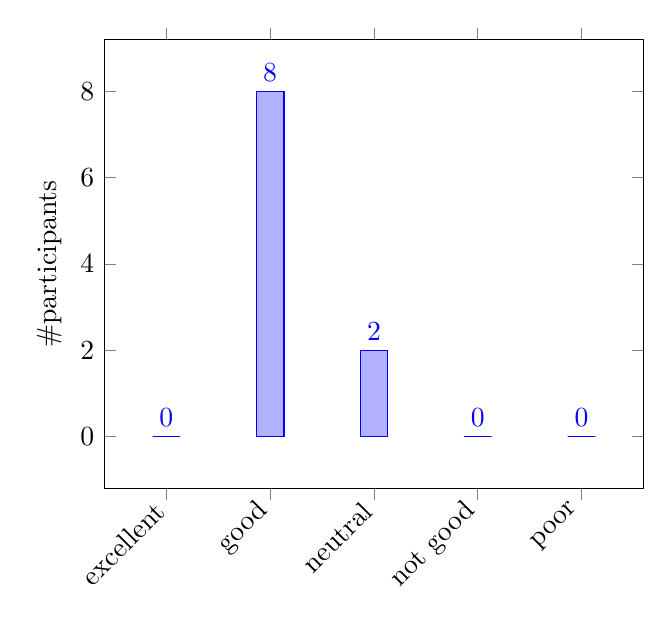
\begin{tikzpicture}
		\begin{axis}
		[
			ybar,
			enlargelimits=0.15,
			legend style={at={(0.5,-0.2)},
			anchor=north,legend columns=-1},
			ylabel={\#participants},
			symbolic x coords={excellent,good,neutral,%
			not good,poor},
			xtick=data,
			nodes near coords,
			nodes near coords align={vertical},
			x tick label style={rotate=45,anchor=east},
		]
			\addplot coordinates {(excellent,0) (good,8) (neutral,2) (not good,0) (poor,0)};
		\end{axis}
	\end{tikzpicture}
\end{document}
